\chapter{Base robotica Otto}

Otto è un robot a guida differenziale, progetto di ricerca del laboratorio di robotica IRALab, dell’Università degli Studi di Milano-Bicocca.

\section{Base robotica VolksBot RT 3}
VolksBot è un kit modulare per la costruzione di robot, progettato per il campo della ricerca e della  prototipazione rapida.
La base robotica è pensata per essere facilmente modificata ed adattata alle proprie esigenze in quanto composta da barre in alluminio combinabili fra di loro. \\
Nello specifico la base robotica utilizzata è composta da due ruote motrici frontali e una ruota basculante di supporto posteriore.
Ciascuna ruota motrice è collegata ad un motore a corrente continua combinato con una riduzione con un rapporto di trasmissione 1:74.
L'intero sistema robotico è alimentato tramite batterie a bordo del veicolo.
\begin{figure}[H]
\centering
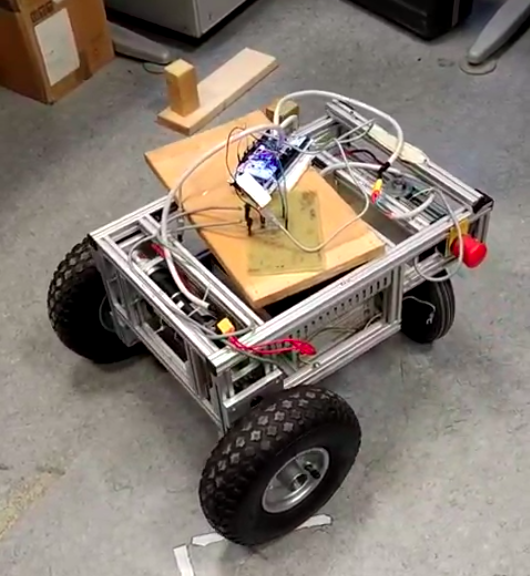
\includegraphics[scale=0.4]{images/otto1.png}
\caption{Base robotica Otto}
\end{figure}

\section{Encoder}
%TODO da rielaborare meglio non so scrivere
Un encoder è dispositivo elettromeccanico in grado di convertire la posizione o il moto angolare in un codice digitale.
Nel nostro caso è stato montato un encoder in quadratura per ogni ruota motrice.
Questo tipo di sensore genera due segnali digitali ad ogni variazione di posizione dell'albero del motore.
Elaborando questi segnali è possibile misurare la distanza percorsa dalle ruote, e anche il verso nel quale si sono mosse.
\begin{figure}[H]
\centering
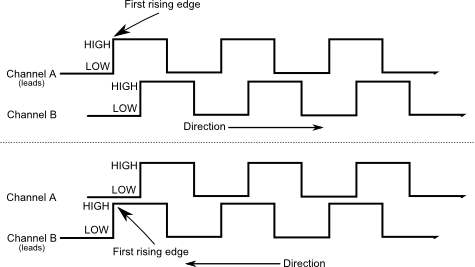
\includegraphics[scale=0.5]{images/quad-encoding-waveform.png}
\caption{Segnali generati dall'encoder.}
\end{figure}

%TODO da rielaborare meglio non so scrivere
\section{Motor driver}
Un motor driver è un dispositivo elettronico necessario per poter controllare i motori DC usando i segnali digitali generati da un microcontrollore.
Il circuito elettronico principale è chiamato H-bridge: permette di controllare la direzione del movimento del motore, di frenarlo o di lasciarlo libero. \\
Il motor driver scelto è Pololu Dual G2: questo dispositivo ha due circuiti H-bridge, così da poter controllare entrambi i motori in modo indipendente e inoltre presenta delle features come la protezione da cortocircuiti.

\section{Microcontrollore}
La scheda di sviluppo scelta è una Nucleo STM32F767ZI, le cui caratteristiche principali sono:
\begin{itemize}
    \item Core Arm® 32-bit Cortex®-M7.
    \item Presenza di un co-processore FPU per i calcoli floating point.
    \item 512 KB di memoria RAM e 2MB di memoria FLASH.
    \item Presenza di un debugger integrato.
\end{itemize}

\begin{figure}[H]
\centering
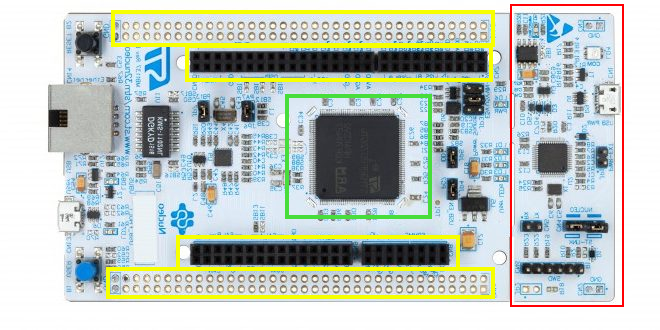
\includegraphics[scale=0.3]{images/nucleo.png}
\caption{La scheda Nucleo.}
\end{figure}

\section{Modulo FTDI}
Per permettere la comunicazione seriale tra microcontrollore e computer è necessario un modulo apposito.
È stato scelto un modulo FTDI FT232RL.
